\begin{card}
	\frametitle{Übung 3: Paradigmen}
	\url{http://people.f4.htw-berlin.de/~hebold/htw/pka/exercises/konzepte-Paradigmen.pdf}
\end{card}

\begin{card}
	Das von-Neumann-Rechnerkonzept (auch von-Neumann-Architektur) zählt zur archetypischen Realisierung des imperativen Programmierparadigmas. Warum?
	\hr
	Imperative Konzept $\ent$ Befehlsorientiert\\
	Fetch, Execute-Zyklus
\end{card}

\begin{card}
	Die Turing-Maschine realisiert ebenfalls das imperativen Programmierparadigma. Warum?
	\hr
	\begin{itemize}
	  \item Überführungsfunktion werden vorher definiert
	  \item Abarbeiten der Behle nacheinander
	  \item Jeder Zustand ist über Befehle verknüpft, vgl. Überführungsfunktion
	\end{itemize}
\end{card}

\begin{card}
	Wieso wird vom von-Neumann-Rechner\textbf{konzept} aber von der Turing-\textbf{Maschine} gesprochen?
	\hr
  \textbf{Konzept:} Abstraktion (Sammlung von Leitsätzen und Prinzipien, Referenzmodell)\\
  \textbf{Maschine:} Konkrete Idee (auch wenn so nicht realisierbar, durch das unendlich lange Band), Maschinenbeschreibung des direkten Programmablaufs
	\begin{figure}[h]
	\centering
	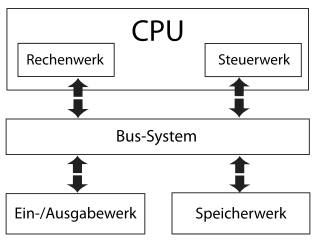
\includegraphics[width=4cm]{Von-Neumann_Architektur}
	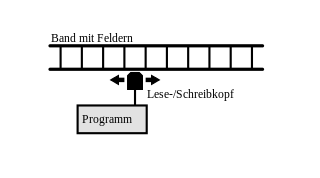
\includegraphics[width=6cm]{Turingmaschine}
	\caption{Von-Neumann, Turing-Maschine}
	\end{figure}
\end{card}

\begin{card}
	Im Zusammenhang mit dem Neumann-Rechnerkonzept ist die Rede vom von-Neumann-Flaschenhals, wenn Nachteile des Konzepts genannte werden.
	\begin{enumerate}[a)]
	\item Was ist darunter zu verstehen?
	\item Gibt es eine vergleichbare Problematik für die Turing-Maschine?
	\end{enumerate}
	\hr
	\begin{enumerate}[a)]
    \item Alle Befehle / Daten müssen seriell durch den Bus (Engpass)
    \item Schreib-/Lesekopf kann pro Zeiteinheit entweder schreiben oder lesen
	\end{enumerate}
\end{card}

\begin{card}
	Nennen Sie wenigstens einen konzeptionellen Unterschied zwischen von-Neumann-Rechnerkonzept und Turing-Maschine.
	\hr
	Von TM ausgehend:

	\begin{itemize}
  \item Daten (Band) und Programme (Tabelle) liegen \textbf{nicht} im selben Speicher
	\item keine Nummerierung/Adressierung eines Feldes auf dem Band
	\item keine Sprungadressen
	\item kann nur 1 Feld gehen pro Befehl
	\end{itemize}
\end{card}

\begin{card}
	Setzt die Turing-Maschine das von-Neumann-Rechnerkonzept um?
	\hr
	\textbf{Nein}, weil
	\begin{itemize}
	\item Bei TM: Daten $\neq$ Programme
	\item TM hat keine Sprungadresse
	\end{itemize}
	\vfill
	oder \textbf{Ja} mit Einschränkungen (vgl. Nein)
	\begin{itemize}
	\item Arbeiten befehlsorientiert
	\item Arbeiten deterministisch
	\end{itemize}
\end{card}

\begin{card}
	Wie könnte das Paradigma der strukturierten Programmierung in das von-Neumann-Rechnerkonzept integriert werden?
	\hr
	Überwachen bzw. Regeln der Sprunganweisungen.\\
	D.h. begrenzter Bereich (Scope) z.B. bei if-Anweisungen
\end{card}

\begin{card}
	Wieso verletzt das Konzept der lokalen static-Variablen in C das Paradigma der funktionalen
	Programmierung?
	\hr
	Funktionsausgabe nur abhängig von Eingabe. D.h. bei gleicher Eingabe, gleiche Ausgabe (Idempotent, Deterministisch).
	\begin{lstlisting}[language=C]
	int f(int i) {
	  // Ausfuehrung bei Objekt-Init,
	  // nicht bei Methodenaufruf
	  static int x = 0;
	  x++;
	  return x+i;
	}
	\end{lstlisting}
	Lokale static Variablen sind über Funktionen hinaus beständig und es entsteht somit eine Abhängigkeit bei wiederholten
	Aufrufen der gleichen Funktion, die Idempotenz wird verletzt.
\end{card}

\begin{card}
	Wieso verletzen Pointer in C das Paradigma der funktionalen Programmierung?
	\hr
	\begin{lstlisting}[language=C]
	int f(int *i) {
	  // Veraendern der Speicheradresse und
	  // somit der Eingabe
	  *i = 1234;
	  ...
	}
	\end{lstlisting}
  \begin{itemize}
    \item Funktionsausgabe nur abhängig von Eingabe.  D.h. bei gleicher Eingabe gleiche Ausgabe.
    \item Nebenläufigkeit (Parallelisierbarkeit) wird verletzt
    \item keine referenzielle Transparenz der Variablen
  \end{itemize}
\end{card}

\begin{card}
	In Java gibt es mit dem Collection-Framework eine Reihe von sogenannten Container-Klassen. Welches objektorientierte Programmierparadigma verletzen Objekte z.B. der Klassen	ArrayList oder Vector?
	\hr
	Es werden Referenzen gespeichert. D.h. die Datenkapselung ist verletzt. Werte müssten unveränderlich (immutable) sein.
	\begin{lstlisting}[language=Java]
	class Dummy{int value;}
	...
	Dummy example = new Dummy()
	ArrayList<Dummy> list = new ArrayList<Dummy>()
	list.add(example);

	// Zugriff auf value ueber 2 Wege:
	example.value = 1;
	list.get(0).value = 2;
	\end{lstlisting}
\end{card}

\begin{card}
	Wie müsste das Funktionskonzept in C beschränkt bzw. erweitert werden, damit es nicht zu Verletzungen des Paradigmas der funktionalen Programmierung kommen kann?
	\hr
	Zustandslosigkeit durch:
	\begin{itemize}
	\item kein static und Pointer
	\item keine Systemaufrufe
	\end{itemize}
\end{card}

\begin{card}
	Das funktionale Programmierparadigma, das die referentielle Transparenz der Variablen fordert, wird in C durch die Zuweisung verletzt.
	\begin{enumerate}[a)]
	\item Wie müssten die Regeln für die Verwendung der Zuweisung geändert werden, damit die	Zuweisung in das funktionale Konzept passt?
	\item Welcher Art von Anweisung entspräche die veränderte Zuweisung dann?
	\end{enumerate}
	\hr
	\begin{enumerate}[a)]
	\item Unveränderliche Variablen, Einmal-Zuweisung, bzw. nur Init.
	\item Konstanteninitialisierung
	\end{enumerate}

\end{card}

\begin{card}
	Die referentielle Transparenz sorgt dafür, dass Programme in rein funktionalen Sprachen	problemlos nebenläufig abgearbeitet werden können.
	\begin{enumerate}[a)]
	\item Erklären Sie den Zusammenhang an einem Beispiel.
	\item Erklären Sie an einem Beispiel den Zusammenhang fehlender referentieller Transparenz und Problemen bei nebenläufig ausgeführten Programmen.
	\end{enumerate}
	\hr
	\begin{enumerate}[a)]
	\item Werte unveränderlich (immutable), d.h. kein Zustand und stark begrenzter Gültigkeitsbereich. Funktionen sind Thread-Safe, da Parameter nicht von außen geändert werden können.\\
	Beispiel: Immutable-Klassen sind automatisch Thread-Safe, parallelisierbar und skalierbar.
\item Objekt-Parameter können während Thread-Unterbrechung über eine Referenz außerhalb der eigentlich Funktion verändert werden und haben somit einen anderen Zustand. Kein Determinismus, Race-Condition (nicht vorhersehbare Zustände) möglich.
	\end{enumerate}
\end{card}

\begin{card}
	Objektorientierte Sprachen kennen sogenannte inline-Funktionen.
	\begin{enumerate}[a)]
	\item Wieso sind inline-Funktionen in objektorientierten Programmiersprachen implementiert?
	\item Sind inline-Funktionen in rein funktionalen Programmiersprachen sinnvoll?
	\item Welches Problem ergibt sich aus inline-Funktionen im Rahmen einer rein funktionalen Sprache?
	\end{enumerate}
	\hr
	\begin{enumerate}[a)]
	\item Performancevorteile, da weniger Overhead durch Stackmanagement
	\item Ja, erhöhen Geschwindigkeit
	\item Rekursionen können nicht aufgelöst werden. Daher nur als Zusatz, nicht als Ersatz für normale Funktionen.
	\end{enumerate}
\end{card}

\begin{card}
	Angenommen in C würden innerhalb von parametrisierten Makros Zuweisungen nicht mehr	zugelassen sein.\\
	Inwiefern verletzen Makros dann trotzdem weiterhin Paradigmen der funktionalen Programmierung?
	\hr
	Variablen sind außerhalb vom Makro gültig, d.h. vor oder nach dem Aufruf / Ersetzung.\\
	Durch die Textersetzung können Variablen(namen) genutzt werden, die erst im nachfolgenden Programm definiert werden. Dadurch ist Idempotenz / Determinismus verletzt.\\
	Beispiel:
	\begin{lstlisting}[language=C]
	#define printX print x
	int x = 100;
	printX(); // Ausgabe: 100
	\end{lstlisting}
\end{card}
